\documentclass{article}
\usepackage{graphicx}
\usepackage[rflt]{floatflt}
\usepackage[T1]{fontenc}
\usepackage{textcomp}
\usepackage[utf8x]{inputenc}
\usepackage{gnuplot-lua-tikz}
\pagestyle{empty}
\begin{document}
\openup.5em
\begin{floatingfigure}{2.9in}
\resizebox{2.5in}{!}{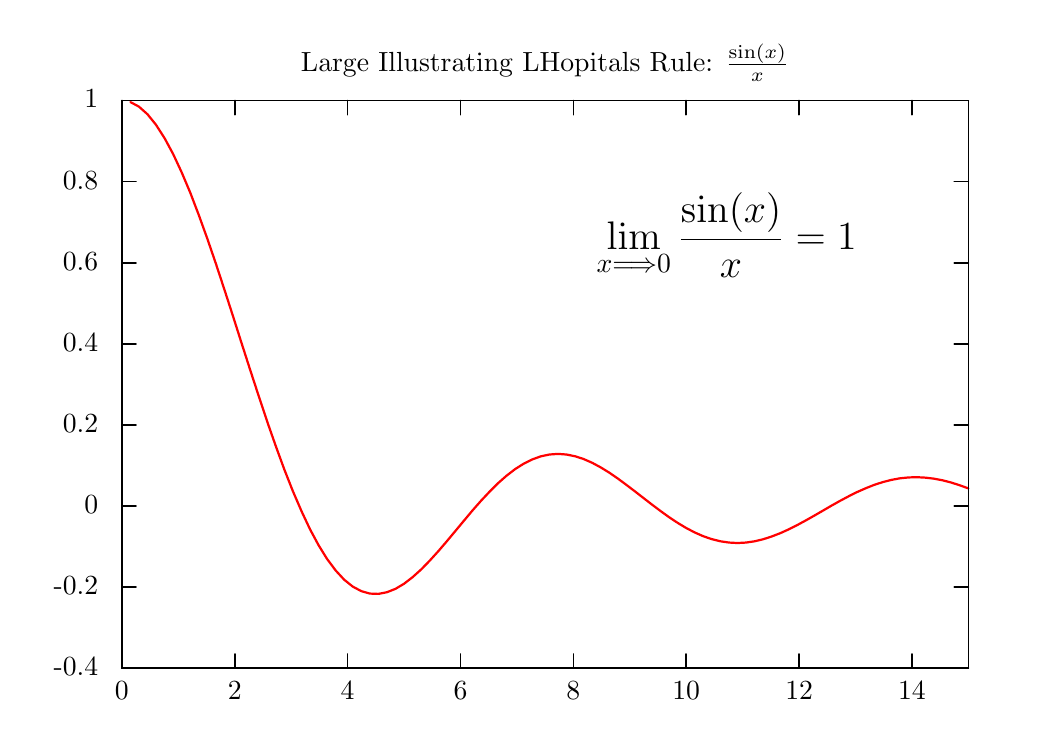
\begin{tikzpicture}[gnuplot]
%% generated with GNUPLOT 4.6p0 (Lua 5.1; terminal rev. 99, script rev. 100)
%% Mon 10 Aug 2015 06:20:26 PM EDT
\path (0.000,0.000) rectangle (12.500,8.750);
\gpcolor{color=gp lt color border}
\gpsetlinetype{gp lt border}
\gpsetlinewidth{1.50}
\draw[gp path] (1.196,0.616)--(1.376,0.616);
\draw[gp path] (11.947,0.616)--(11.767,0.616);
\node[gp node right] at (1.012,0.616) {-0.4};
\draw[gp path] (1.196,1.646)--(1.376,1.646);
\draw[gp path] (11.947,1.646)--(11.767,1.646);
\node[gp node right] at (1.012,1.646) {-0.2};
\draw[gp path] (1.196,2.676)--(1.376,2.676);
\draw[gp path] (11.947,2.676)--(11.767,2.676);
\node[gp node right] at (1.012,2.676) { 0};
\draw[gp path] (1.196,3.706)--(1.376,3.706);
\draw[gp path] (11.947,3.706)--(11.767,3.706);
\node[gp node right] at (1.012,3.706) { 0.2};
\draw[gp path] (1.196,4.735)--(1.376,4.735);
\draw[gp path] (11.947,4.735)--(11.767,4.735);
\node[gp node right] at (1.012,4.735) { 0.4};
\draw[gp path] (1.196,5.765)--(1.376,5.765);
\draw[gp path] (11.947,5.765)--(11.767,5.765);
\node[gp node right] at (1.012,5.765) { 0.6};
\draw[gp path] (1.196,6.795)--(1.376,6.795);
\draw[gp path] (11.947,6.795)--(11.767,6.795);
\node[gp node right] at (1.012,6.795) { 0.8};
\draw[gp path] (1.196,7.825)--(1.376,7.825);
\draw[gp path] (11.947,7.825)--(11.767,7.825);
\node[gp node right] at (1.012,7.825) { 1};
\draw[gp path] (1.196,0.616)--(1.196,0.796);
\draw[gp path] (1.196,7.825)--(1.196,7.645);
\node[gp node center] at (1.196,0.308) { 0};
\draw[gp path] (2.629,0.616)--(2.629,0.796);
\draw[gp path] (2.629,7.825)--(2.629,7.645);
\node[gp node center] at (2.629,0.308) { 2};
\draw[gp path] (4.063,0.616)--(4.063,0.796);
\draw[gp path] (4.063,7.825)--(4.063,7.645);
\node[gp node center] at (4.063,0.308) { 4};
\draw[gp path] (5.496,0.616)--(5.496,0.796);
\draw[gp path] (5.496,7.825)--(5.496,7.645);
\node[gp node center] at (5.496,0.308) { 6};
\draw[gp path] (6.930,0.616)--(6.930,0.796);
\draw[gp path] (6.930,7.825)--(6.930,7.645);
\node[gp node center] at (6.930,0.308) { 8};
\draw[gp path] (8.363,0.616)--(8.363,0.796);
\draw[gp path] (8.363,7.825)--(8.363,7.645);
\node[gp node center] at (8.363,0.308) { 10};
\draw[gp path] (9.797,0.616)--(9.797,0.796);
\draw[gp path] (9.797,7.825)--(9.797,7.645);
\node[gp node center] at (9.797,0.308) { 12};
\draw[gp path] (11.230,0.616)--(11.230,0.796);
\draw[gp path] (11.230,7.825)--(11.230,7.645);
\node[gp node center] at (11.230,0.308) { 14};
\draw[gp path] (1.196,7.825)--(1.196,0.616)--(11.947,0.616)--(11.947,7.825)--cycle;
\node[gp node center] at (6.571,8.287) {Large Illustrating LHopitals Rule: $\frac{\sin(x)}{x}$};
\node[gp node left] at (7.109,6.023) {\Large$\displaystyle \lim_{x\Longrightarrow0}\frac{\sin(x)}{x}=1$};
\gpcolor{color=gp lt color 0}
\gpsetlinetype{gp lt plot 0}
\gpsetlinewidth{2.00}
\draw[gp path] (1.305,7.805)--(1.413,7.747)--(1.522,7.650)--(1.630,7.516)--(1.739,7.346)%
  --(1.848,7.144)--(1.956,6.912)--(2.065,6.654)--(2.173,6.371)--(2.282,6.069)--(2.391,5.751)%
  --(2.499,5.422)--(2.608,5.085)--(2.716,4.745)--(2.825,4.406)--(2.934,4.072)--(3.042,3.747)%
  --(3.151,3.436)--(3.259,3.140)--(3.368,2.864)--(3.477,2.611)--(3.585,2.381)--(3.694,2.178)%
  --(3.802,2.003)--(3.911,1.857)--(4.019,1.740)--(4.128,1.652)--(4.237,1.594)--(4.345,1.563)%
  --(4.454,1.559)--(4.562,1.580)--(4.671,1.623)--(4.780,1.688)--(4.888,1.771)--(4.997,1.869)%
  --(5.105,1.980)--(5.214,2.100)--(5.323,2.227)--(5.431,2.357)--(5.540,2.488)--(5.648,2.617)%
  --(5.757,2.741)--(5.866,2.857)--(5.974,2.965)--(6.083,3.061)--(6.191,3.144)--(6.300,3.213)%
  --(6.409,3.267)--(6.517,3.306)--(6.626,3.329)--(6.734,3.337)--(6.843,3.329)--(6.952,3.307)%
  --(7.060,3.272)--(7.169,3.224)--(7.277,3.166)--(7.386,3.099)--(7.495,3.024)--(7.603,2.944)%
  --(7.712,2.861)--(7.820,2.777)--(7.929,2.693)--(8.038,2.611)--(8.146,2.533)--(8.255,2.461)%
  --(8.363,2.396)--(8.472,2.339)--(8.581,2.291)--(8.689,2.254)--(8.798,2.227)--(8.906,2.211)%
  --(9.015,2.205)--(9.124,2.211)--(9.232,2.227)--(9.341,2.253)--(9.449,2.288)--(9.558,2.330)%
  --(9.666,2.379)--(9.775,2.434)--(9.884,2.493)--(9.992,2.554)--(10.101,2.617)--(10.209,2.680)%
  --(10.318,2.741)--(10.427,2.799)--(10.535,2.853)--(10.644,2.901)--(10.752,2.944)--(10.861,2.979)%
  --(10.970,3.007)--(11.078,3.027)--(11.187,3.038)--(11.295,3.041)--(11.404,3.035)--(11.513,3.022)%
  --(11.621,3.001)--(11.730,2.973)--(11.838,2.938)--(11.947,2.899);
\gpcolor{color=gp lt color border}
\gpsetlinetype{gp lt border}
\gpsetlinewidth{1.50}
\draw[gp path] (1.196,7.825)--(1.196,0.616)--(11.947,0.616)--(11.947,7.825)--cycle;
%% coordinates of the plot area
\gpdefrectangularnode{gp plot 1}{\pgfpoint{1.196cm}{0.616cm}}{\pgfpoint{11.947cm}{7.825cm}}
\end{tikzpicture}
%% gnuplot variables
}
\end{floatingfigure}
\noindent The figure to the right provides an illustration of
L'H\^o\-pi\-tal's Rule. Recall that this rule can be applied when
taking the limit as $x\longrightarrow x_a$ of a ratio of two
functions where the ratio approaches the indeterminate form
$\frac{0}{0}$; in the case where both functions are
differentiable at $x_a$, the ratio approaches the ratio of their
derivatives. In the case illustrated both $\sin(x)$ and $x
\longrightarrow0$ as we approach the origin, but the ratio of their
derivatives, $\frac{\cos(x)}{1} \longrightarrow 1$. L'H\^opital's
Rule also applies in the case of the
indeterminate form $\frac{\infty}{\infty}$.
\end{document}

